\documentclass{article}

\usepackage{parskip}
\usepackage{geometry}
\usepackage{graphicx}
\RequirePackage[dvipsnames]{xcolor}
\definecolor{darkblue}{rgb}{0, 0, 0.5}
\definecolor{darkred}{HTML}{8b0000}
\usepackage{hyperref}
\hypersetup{
  colorlinks,
  linkcolor=darkred,
  citecolor=darkred,
  urlcolor=darkred
}

\title{Task Specification}
\author{Giulio Starace \and Niklas Höpner} \begin{document} \maketitle

We are interested in formalizing the scenario of \textit{task specification}. This is the scenario
in which a \textit{requester} $R$ specifies a \textit{task} to be performed by an \textit{actor} $A$.
Note that this generalizes self-proposed tasks, in which the actor is also the requester $A=R$.

\section{Preliminary Definitions}

\subsection{Task Specification}

We view task specification as being formed by two steps from the requester:
\begin{enumerate}
	\item \textbf{Task formulation}: The requester forms a high-level representation $\mathcal{T}$ of
	      the ideal trajectory of state-action pairs $T$, corresponding to the task they would like to be
	      performed.
	\item \textbf{Task communication}: The requester somehow communicates this representation to the
	      actor. This is trivial in the case where requester and actor are the same agent.
\end{enumerate}

\subsection{Task Performance}

Task specification will always be closely linked to \textit{task performance} from the actor, as
ultimately they both share the overarching goal of realizing a certain task. We see task performance
as being composed of the following two steps:

\begin{enumerate}
	\item \textbf{Task understanding}: The actor takes the communication from the requester and forms
	      some inner representation $\mathcal{I}$ used for choosing which actions to execute when seeing
	      a given state so to successfully perform the task\footnote{This could correspond to the process
		      of learning a policy $\pi(a|s)$ in RL, but I am not 100\% sure.}.
	\item \textbf{Action execution}: The actor executes the sequence of actions necessary to produce
	      a trajectory $T$ of state-action pairs which matches some high-level representation of the
	      desired trajectory $\mathcal{T}$ as idealized by the requester.
\end{enumerate}


\section{Evaluation}

Evaluation of task specification is a complex topic, as it is inherently entangled with the
evaluation of task performance. A successful task specification is one which leads to an accurate
task understanding, i.e. where the mutual information between $\mathcal{I}$ and $\mathcal{T}$ is
maximized\footnote{Epistemic status on the mutual information note: this is a guess}. High quality
task specification can improve task performance, but is not the only ingredient for success, as the
actor may be limited in other ways.

First we note that the extent of the match between the executed $T$ and the requested $\mathcal{T}$
(0 being completely dissatisfied, 1 being complete satisfaction) is determined by some evaluating
function $m$ known (consciously or subconsciously) by the requester\footnote{I believe some
	treatment of uncertainty may be warranted here: the requester is never 100\% certain about what
	they want.}:

\begin{equation}
	m(\mathcal{T}, T) \mapsto [0, 1].
\end{equation}

Note that it may be in the actor's interest to estimate this function in some way.

We work with high-level representations of trajectories rather than raw trajectories because it can
occur that the requester does not know exactly what sequence of state-action pairs they want, and
are typically more interested in higher level desiderata anyway.

\section{Additional Notes}

\subsection{Methods of Task Communication}

We can think of a few ways a requester may specify tasks to external actors:
\begin{enumerate}
	\item Through language: this is how we typically specify tasks in a human-requester human-actor
	      setting.
	\item Through demonstrations: consider the case of showing a baby how to walk by walking
	      yourself.
	\item Through preferences: for instance by comparing trajectory segments and ranking them by how much you like them.
	\item Through rewards and penalties: consider Pavlovian training of animals or reinforcement
	      learning. We note that the reward function is not necessarily well aligned with $m$.
	\item Other methods: formal language, etc.
	\item Some combination of the above
\end{enumerate}

\subsection{Granularity of specification}

We note that different modes of communication will be more or less granular in their ability to
specify tasks, where the spectrum of granularity ranges from actions on one extreme to high level
representations of trajectories on the other extreme. While in principle natural language may be
used to express even the most granular of details, it is most naturally used to communicate high
level desiderata and descriptions of behaviour. Rewards on the other hand may become too ambiguous
or low-bandwidth for communicating intent at this level of abstraction, and may be more suited for
communicating which action is optimal at a given state. Demonstrations seem to fall between the two. We refer to
Fig.~\ref{fig:granularity} for a visual illustration.

\begin{figure}[ht]
	\centering
	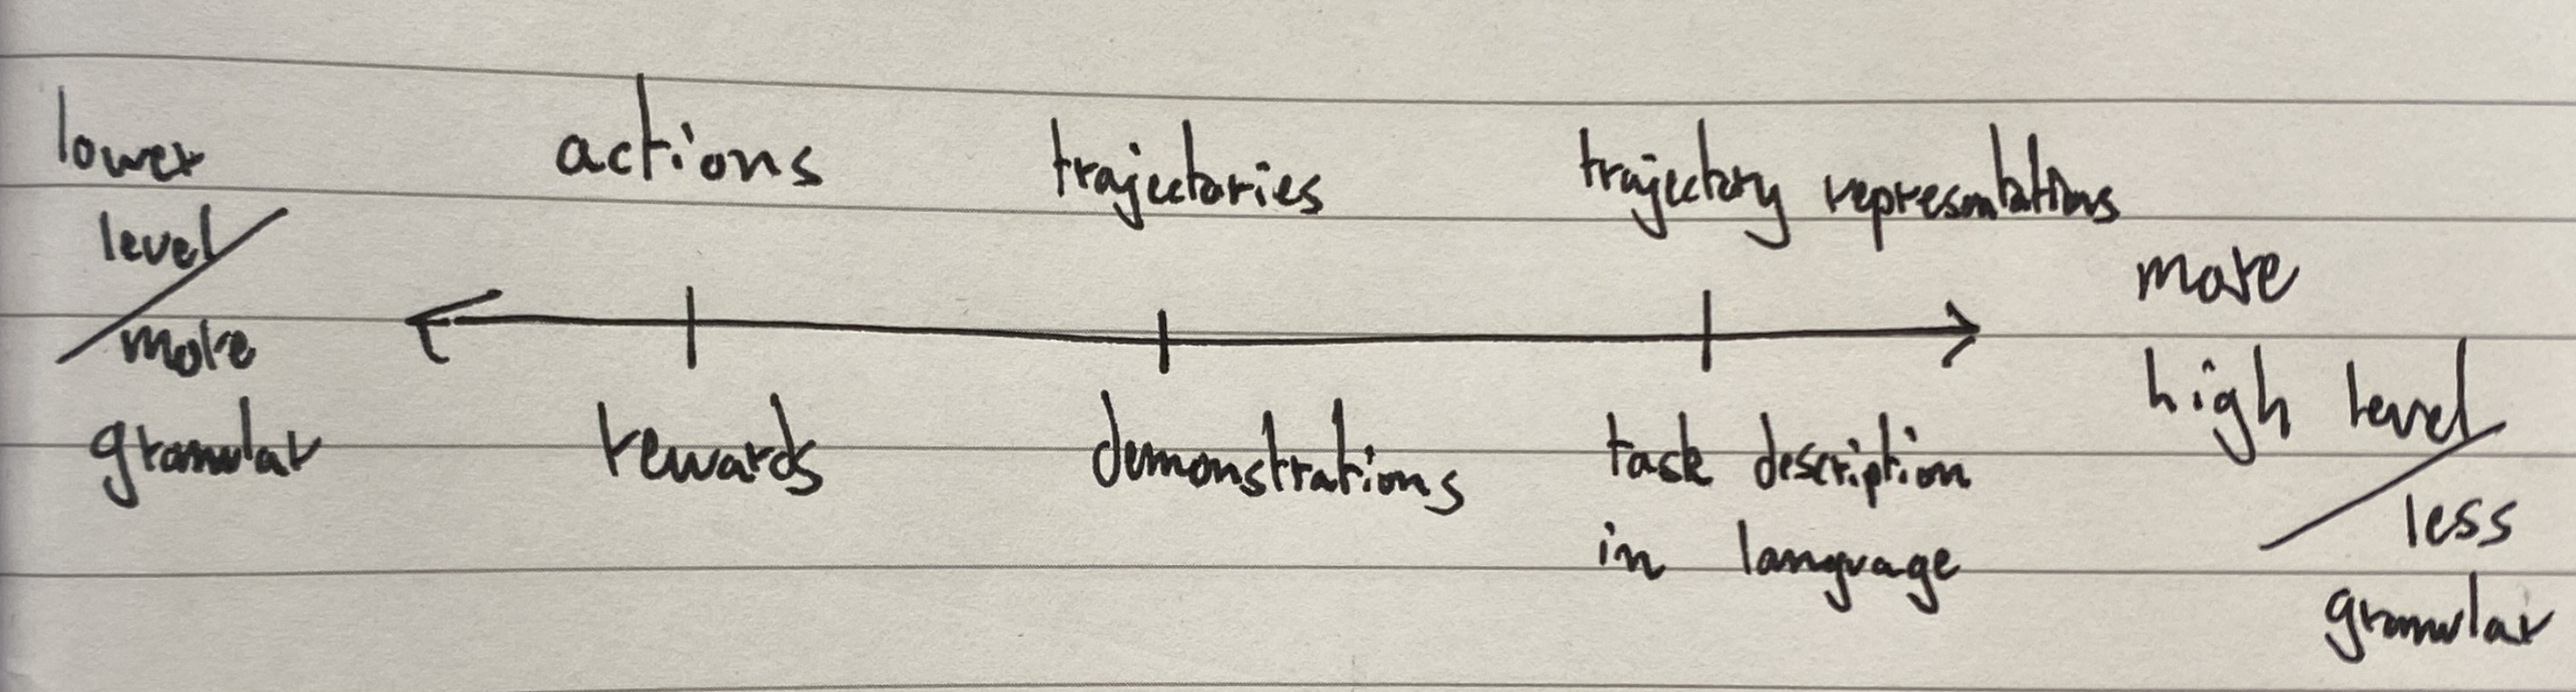
\includegraphics[width=\textwidth]{img/IMG_9800.jpg}
	\caption{Different levels of granularity of specification, and which communication methods and
		abstraction level they most naturally map to}
	\label{fig:granularity}
\end{figure}

\begin{figure}[ht]
	\centering
	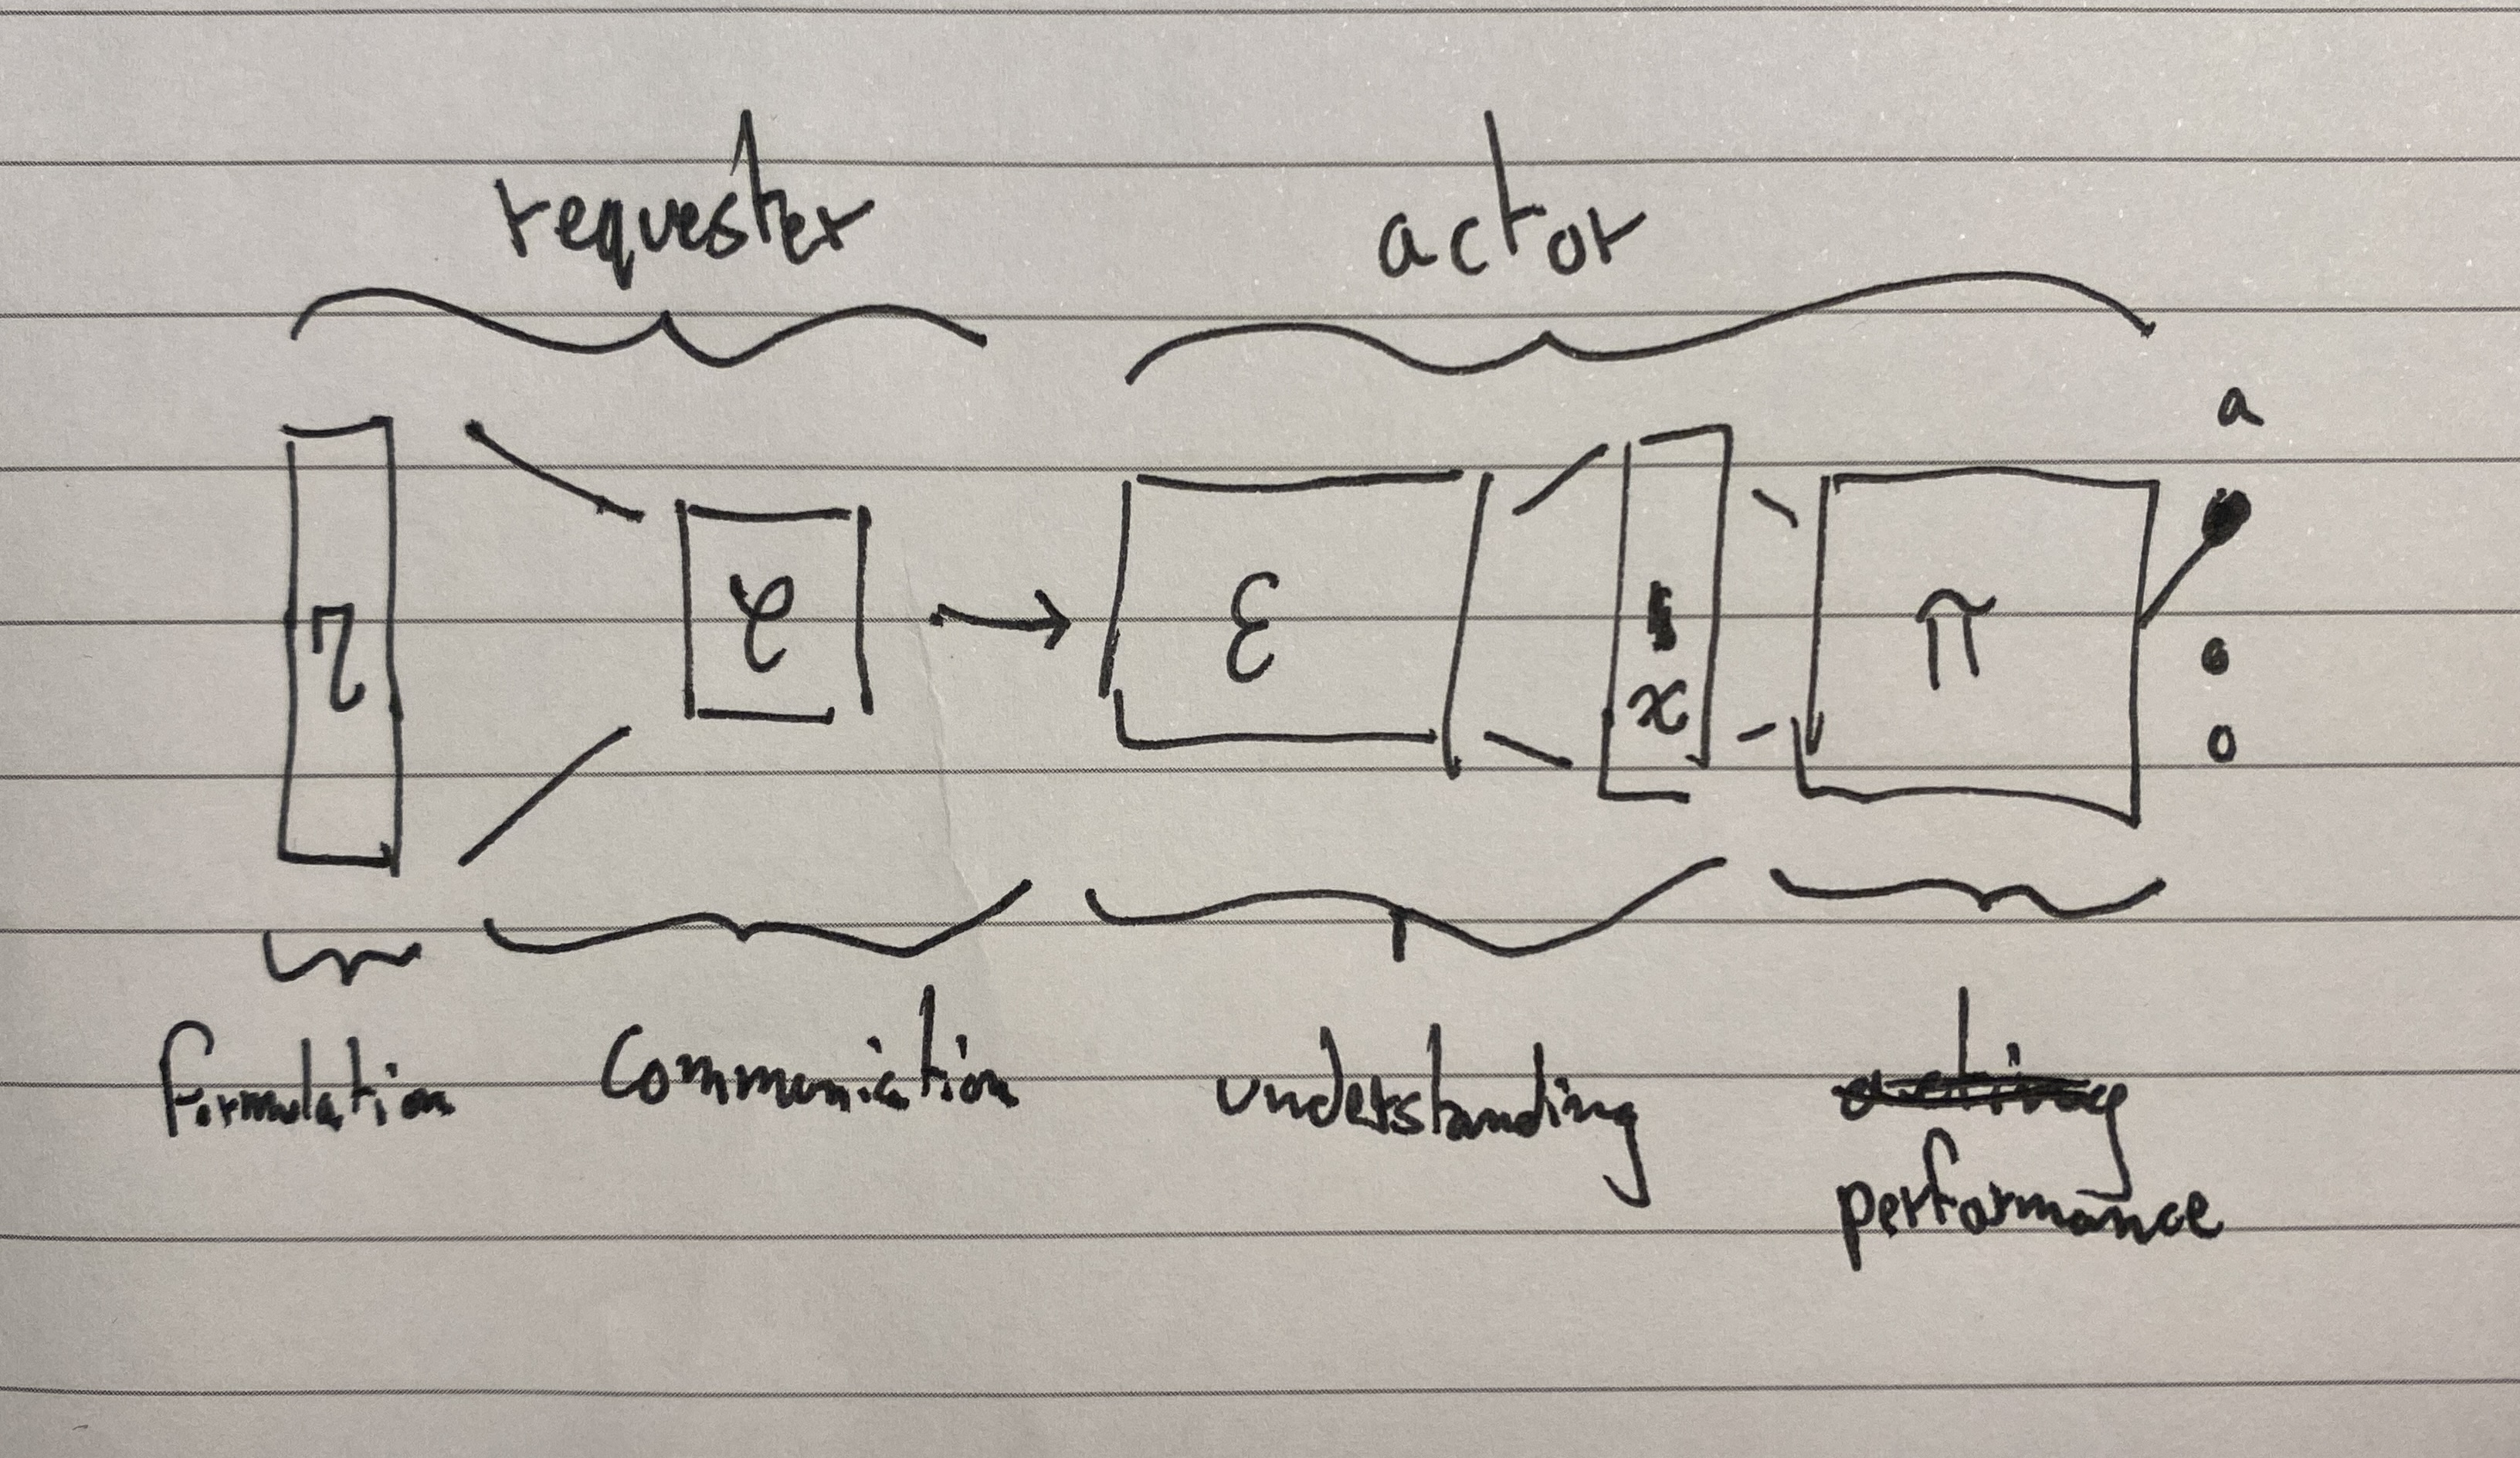
\includegraphics[width=\textwidth]{img/IMG_9745.jpg}
	\caption{Rough sketch of our formalism for the case of natural language task communication: The
		requester formulates an ideal trajectory of the desired outcome, $\mathcal{T}$. They then
		communicate this task by  mapping $\mathcal{T}$ to a representation in natural language $\varphi$.
		The actor receives $\varphi$ and ``understands'' it, using an encoder $\varepsilon$ to map it to
		some internal representation $x$ to be used by their policy $\pi$ along with other data (such as
		environment observations) to perform actions.}
	\label{fig:rough_sketch}
\end{figure}

\end{document}


